\documentclass[11pt]{beamer}
\setbeamercovered{transparent}
\usetheme[progressbar=frametitle]{metropolis}
\usepackage[french]{babel}
\usepackage{datetime, xcolor, amsthm, tikz}
\usepackage[makeroom]{cancel}
\usepackage[french]{algorithm2e}

\usetikzlibrary{calc, fit, decorations.pathreplacing}

\title{Stage de Master IGIS ITA}
\subtitle{Bioinformatique, découverte de motifs entre des ensembles de fragments d’ADN}
\date{\formatdate{03}{07}{2017}}
\author{Gabriel Toublanc}
\institute{
  Université de Rouen, U.F.R des Sciences et Techniques de Saint-Étienne-du-Rouvray, LITIS EquipeTIBS\medskip\\
  Encadrants : Thierry Lecroq et Arnaud Lefebvre
}
\titlegraphic{%
  \vspace{73mm}
  \begin{tabular}{cccc}
    \begin{minipage}[b]{0.2\textwidth}\centering
\includegraphics[height=8mm]{logo_normandie}\end{minipage} &
    \begin{minipage}[b]{0.2\textwidth}\centering
\includegraphics[height=8mm]{logo_univ_rouen}\end{minipage} &
    \begin{minipage}[b]{0.2\textwidth}\centering
\includegraphics[height=8mm]{logo_ufr_sciences}\end{minipage} &
    \begin{minipage}[b]{0.2\textwidth}\centering
\includegraphics[height=7mm]{logo_litis}\end{minipage}
  \end{tabular}
}
\newcommand{\pauseline}{\\\pause\bigskip}
\newcommand{\setcolor}[2]{\textcolor{#1}{#2}}
\newcommand{\red}[1]{\setcolor{red}{#1}}
\newcommand{\green}[1]{\setcolor{green}{#1}}
\newcommand{\blue}[1]{\setcolor{blue}{#1}}

\newtheorem{thmgt}{Théorème}
\newtheorem{defgt}{Définition}
\newtheorem{lemgt}{Lemme}
\newtheorem{corgt}{Corollaire}
\newtheorem{progt}{Proposition}

\renewcommand\qedsymbol{$\blacksquare$}

\begin{document}
\maketitle
\metroset{block=fill}

\begin{frame}[fragile]{Table des matières}
  \Large
  \begin{enumerate}[<+-| alert@+>]
    \item Introduction
    \item K-mers et k-mers espacés
    \item Implémentations
    \item Résultats obtenus
    \item Conclusion
  \end{enumerate}
\end{frame}

\section{Introduction}
\begin{frame}[fragile]{Le séquençage ADN}
  \setbeamercovered{invisible}
  \begin{overprint}
    \begin{center}\begin{tabular}{cc}
      \onslide<1->{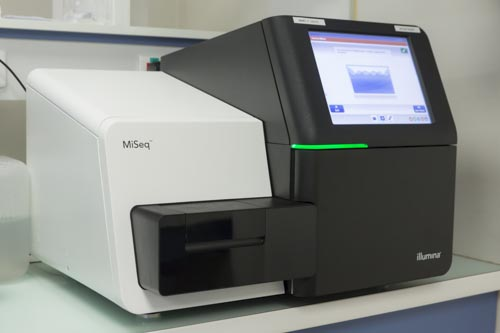
\includegraphics[height=30mm]{sequenceur_illumina}} &
      \onslide<2->{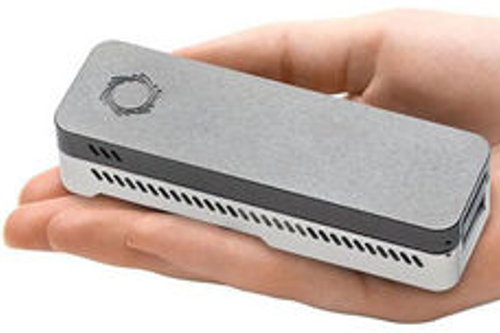
\includegraphics[height=30mm]{sequenceur_minion}}
    \end{tabular}\end{center}
    \begin{itemize}[<+-| alert@+>]
      \item Lectures courtes (depuis 2005, 20 à 300 nucléotides, Illumina, Roche, ...)
      \item Lectures longues (depuis 2010, 3k à 20k nucléotides, Oxford Nanopore, Pacific Biosciences)
    \end{itemize}
  \end{overprint}
\end{frame}

\begin{frame}[fragile]{Alignement et assemblage}
  \setbeamercovered{invisible}
  \begin{figure}
    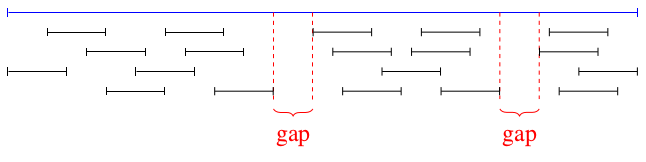
\includegraphics[width=80mm]{alignement_courts}
    \caption{Alignement sur les lectures courtes}
  \end{figure}
  \pause
  \begin{figure}
    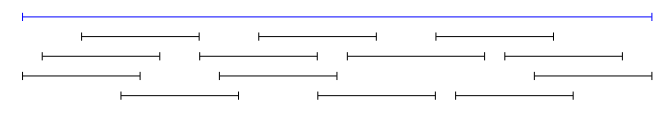
\includegraphics[width=80mm]{alignement_longs}
    \caption{Alignement sur les lectures longues}
  \end{figure}
\end{frame}

\begin{frame}[fragile]{Alignement et assemblage}
  \setbeamercovered{invisible}
  \begin{figure}
    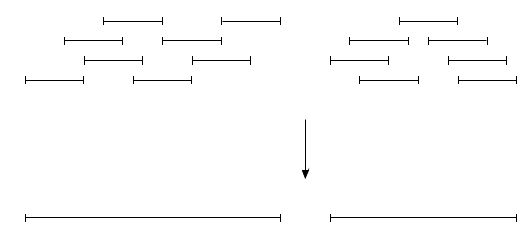
\includegraphics[width=55mm]{assemblage_courts}
    \caption{Assemblage sur les lectures courtes}
  \end{figure}
  \pause
  \begin{figure}
    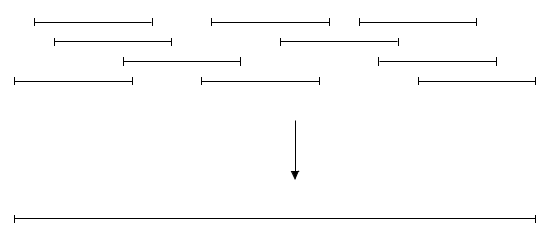
\includegraphics[width=55mm]{assemblage_longs}
    \caption{Assemblage sur les lectures longues}
  \end{figure}
\end{frame}

\begin{frame}[fragile]{Corrections des lectures longues}
  \textbf{Lectures courtes} : problème de couverture du génome\medskip\pause\\
  \textbf{Lectures longues} : problème de taux d'erreur de lecture\pause
  \begin{itemize}[<+-| alert@+>]
    \item Oxford Nanopore : 30\% d'erreurs
    \item Pacific BioSciences : 15\% d'erreurs
  \end{itemize}\pause
  \textbf{Une solution} : corriger les lectures longues avec les lectures courtes (< 1\% d'erreur, voir \textbf{HG-CoLoR}\footnote{Pierre Morisse, Thierry Lecroq and Arnaud Lefebvre\cite{Morisse2017}}).\medskip\pause\\
  \textbf{Notre solution} : tenter de corriger les lectures longues directement.
\end{frame}

\section{$K$-mers et $k$-mers espacés}
\begin{frame}[fragile]{Extraction des $k$-mers}
  Les $k$-mers sont des facteurs de longueur $k$ de séquences d'ADN.\medskip\\\pause
  \textbf{Ex} : Avec la séquence $s = AACCGGTT$ de longueur $L$, on obtient les $k$-mers de longueur $6$ ($6$-mers) suivants :\\\pause
  \begin{center}\begin{tikzpicture}
    \coordinate (s) at (0, 2);
    \foreach \xi [count=\i] in {\mathbf{k_1 :}, A, A, C, C, G, G, T, T} {
      \node[minimum size=5mm] (x\i) at (s) {$\xi$};
      \coordinate (s) at ($(s) + (0.8, 0)$);
    }
    \node[draw,rectangle,red,fit=(x2) (x7)] {};
    \pause
    \coordinate (s) at (0, 1);
    \foreach \yi [count=\i] in {\mathbf{k_2 :}, A, A, C, C, G, G, T, T} {
      \node[minimum size=5mm] (y\i) at (s) {$\yi$};
      \coordinate (s) at ($(s) + (0.8, 0)$);
    }
    \node[draw,rectangle,red,fit=(y3) (y8)] {};
    \pause
    \coordinate (s) at (0, 0);
    \foreach \zi [count=\i] in {\mathbf{k_3 :}, A, A, C, C, G, G, T, T} {
      \node[minimum size=5mm] (z\i) at (s) {$\zi$};
      \coordinate (s) at ($(s) + (0.8, 0)$);
    }
    \node[draw,rectangle,red,fit=(z4) (z9)] {};
  \end{tikzpicture}\end{center}
\end{frame}
\begin{frame}[fragile]{$K$-mers espacés}
  Les $k$-mers espacés sont des $k$-mers discontinus.\pause\medskip\\
  On utilise un motif $m$ composé de zéros et de uns pour les représenter, où chaque zéro correspond à une insertion/délétion.\medskip\pause\\
  \textbf{Ex} : Avec la séquence $s=AACCGGTT$...\pause
  \begin{itemize}[<+-| alert@+>]
    \item et le motif $m=10100111$, on obtient le $5$-mers espacé à délétion $ACGTT$
    \item et le motif $m=10011$, on obtient les $5$-mers espacé à insertion $\{AAAAC, AACACC...\}$
  \end{itemize}
\end{frame}
\begin{frame}[fragile]{$K$-mers espacés à délétion}
  Utilisé afin de simuler des corrections aux erreurs d'insertions sur les lectures longues.\medskip\\\pause
  \textbf{Ex} : Avec la séquence $s = AACCGGTT$ et le motif $m = 111011$, on obtient les $5$-mers espacés suivants :\\\pause
  \begin{center}\begin{tikzpicture}
    \coordinate (s) at (0, 2);
    \foreach \xi [count=\i] in {\mathbf{k_1 :}, A, A, C, \xcancel{C}, G, G, T, T} {
      \node[minimum size=5mm] (x\i) at (s) {$\xi$};
      \coordinate (s) at ($(s) + (0.8, 0)$);
    }
    \node[draw,rectangle,red,fit=(x2) (x4)] {};
    \node[draw,rectangle,red,fit=(x6) (x7)] {};
    \pause
    \coordinate (s) at (0, 1);
    \foreach \yi [count=\i] in {\mathbf{k_2 :}, A, A, C, C, \xcancel{G}, G, T, T} {
      \node[minimum size=5mm] (y\i) at (s) {$\yi$};
      \coordinate (s) at ($(s) + (0.8, 0)$);
    }
    \node[draw,rectangle,red,fit=(y3) (y5)] {};
    \node[draw,rectangle,red,fit=(y7) (y8)] {};
    \pause
    \coordinate (s) at (0, 0);
    \foreach \zi [count=\i] in {\mathbf{k_3 :}, A, A, C, C, G, \xcancel{G}, T, T} {
      \node[minimum size=5mm] (z\i) at (s) {$\zi$};
      \coordinate (s) at ($(s) + (0.8, 0)$);
    }
    \node[draw,rectangle,red,fit=(z4) (z6)] {};
    \node[draw,rectangle,red,fit=(z8) (z9)] {};
  \end{tikzpicture}\end{center}
\end{frame}
\begin{frame}[fragile]{$K$-mers espacés à insertion}
  Utilisé afin de simuler des corrections aux erreurs de délétion sur les lectures longues.\medskip\\\pause
  $\mathbf{(L - k + 1)*4^t}$ $k$-mers espacés à insertion possibles, avec $t = $nombre de 0 dans le motif.\medskip\\\pause
  \textbf{Ex} : Avec la séquence $\mathbf{s = AACCGGTT}$ et le motif $\mathbf{m = 111011}$, on obtient les $6$-mers espacés suivants :\\\pause
  \begin{center}\begin{tikzpicture}
    \coordinate (s) at (0, 3);
    \foreach \xi [count=\i] in {$\mathbf{k_1 :}$, $A$, $A$, $C$, \tiny$\underbrace{A, C, G, T}_{}$, $C$, $G$, $G$, $T$, $T$} {
      \node[minimum size=5mm] (x\i) at (s) {\xi};
      \coordinate (s) at ($(s) + (0.8, 0)$);
    }
    \node[draw,rectangle,red,fit=(x2) (x7)] {};
    \pause
    \coordinate (s) at (0, 2);
    \foreach \yi [count=\i] in {$\mathbf{k_2 :}$, $A$, $A$, $C$, $C$, \tiny$\underbrace{A, C, G, T}_{}$, $G$, $G$, $T$, $T$} {
      \node[minimum size=5mm] (y\i) at (s) {\yi};
      \coordinate (s) at ($(s) + (0.8, 0)$);
    }
    \node[draw,rectangle,red,fit=(y3) (y8)] {};
    \pause
    \coordinate (s) at (0, 1);
    \foreach \zi [count=\i] in {$\mathbf{k_3 :}$, $A$, $A$, $C$, $C$, $G$, \tiny$\underbrace{A, C, G, T}_{}$, $G$, $T$, $T$} {
      \node[minimum size=5mm] (z\i) at (s) {\zi};
      \coordinate (s) at ($(s) + (0.8, 0)$);
    }
    \node[draw,rectangle,red,fit=(z4) (z9)] {};
    \pause
    \coordinate (s) at (0, 0);
    \foreach \mi [count=\i] in {$\mathbf{k_4 :}$, $A$, $A$, $C$, $C$, $G$, $G$, \tiny$\underbrace{A, C, G, T}_{}$, $T$, $T$} {
      \node[minimum size=5mm] (m\i) at (s) {\mi};
      \coordinate (s) at ($(s) + (0.8, 0)$);
    }
    \node[draw,rectangle,red,fit=(m5) (m10)] {};
  \end{tikzpicture}\end{center}
\end{frame}

\section{Implémentations}
\begin{frame}[fragile]{Implémentation : kmersDel}
  \textbf{Jellyfish}\footnote{Guillaume Marcais and Carl Kingsford\cite{Marcais2011}} est la référence pour l'extraction de $k$-mers contigus.\medskip\\\pause
  Pour les $k$-mers espacés à délétion, l'outil \textbf{GkAmpi}\footnote{Alban Mancheron\cite{Mancheron}} est en cours de développement.\medskip\\\pause
  Les programmes kmersDel et kmersExpand, développés en C++11 \textit{multi-thread}, traitent les $k$-mers à délétion et insertion.\medskip\\\pause
  Deux versions de kmersDel existent:\pause
  \begin{itemize}[<+-| alert@+>]
    \item Une renommée kmersCount, favorisant la vitesse en dépit de l'utilisation de la mémoire
    \item L'autre, kmersDel, est moins efficace mais peut être couplé à \textbf{Jellyfish} sur n'importe quelle longueur de $k$-mers
  \end{itemize}\bigskip
\end{frame}

\begin{frame}[fragile]{Implémentation : kmersDel}
  \scriptsize
  \begin{algorithm}[H]{
    \Entree{table\_hachage $table$, mots $lectures$, mot $motif$, entier $k$}
    \pause
    \PourCh{$lecture$ de $lectures$}{
      \pause
      \Pour{$i = 0;\ i + k \le |lecture|;\ i += 1$}{
        $kmerEntier = 0$\;
        $kmer = ""$\;
        \pause
        \Pour{$j = 0;\ j < k;\ j += 1$}{
          \lSi{$motif[j] \ne 0$}{$kmer = kmer + lecture[i + j]$}
        }
        \pause
        \PourCh{$nucleotide$ de $kmer$}{
          $kmerEntier *= 4$\;
          \Suivant{valeur de $nucleotide$}{
            \lCas{A}{}
            \lCas{C}{$kmerEntier += 1$}
            \lCas{G}{$kmerEntier += 2$}
            \lCas{T}{$kmerEntier += 3$}
          }
        }
        \pause
        $table[kmerEntier] += 1$\;
      }
    }
  }\end{algorithm}
  \normalsize
\end{frame}

\begin{frame}[fragile]{Implémentation : kmersExpand}
  \textbf{\normalsize kmersExpand}
  \pause
  \scriptsize
  \begin{algorithm}[H]{
    \Entree{mots $lectures$, mot $motif$, entier $k$}
    \pause
    \PourCh{$lecture$ de $lectures$}{
      \pause
      \Pour{$i = 0;\ i + k \le |lecture|;\ i += 1$}{
        $kmer = lecture[i:k]$\;
        $kmersExpandRec(kmer, motif, 0)$\;
      }
    }
  }\end{algorithm}
  \pause
  \textbf{\normalsize kmersExpandRec}
  \begin{algorithm}[H]{
    \Entree{mot $kmer$, mot $nvKmer$, mot $motif$, entier $posMotif$, entier $posKmer$}
    \pause
    \lSi{$posSeed == |motif|$}{$affiche(nvKmer)$}
    \pause
    \lSinonSi{$motif[posMotif] \ne 0$}{$kmersExpandRec(kmer, nvKmer + kmer[posKmer], posMotif+1, posKmer+1)$}
    \pause
    \Sinon{
      $kmersExpandRec(kmer, nvKmer + A, posMotif+1, posKmer)$\;
      $kmersExpandRec(kmer, nvKmer + C, posMotif+1, posKmer)$\;
      $kmersExpandRec(kmer, nvKmer + G, posMotif+1, posKmer)$\;
      $kmersExpandRec(kmer, nvKmer + T, posMotif+1, posKmer)$\;
    }
  }\end{algorithm}
  \normalsize
\end{frame}

\begin{frame}[fragile]{Mots Minimaux Absents (MAW)}
  \begin{defgt}
    Un mot minimal absent d'une séquence est un mot absent dont les facteurs propres (plus long suffixe propre et plus long préfixe propre) sont tous présents dans la séquence.
  \end{defgt}
  \pause
  Avec la séquence \only<-2>{$s = AACACACC$}\only<3>{$s = \red{AACAC}ACC$}\only<4>{$s = AAC\red{ACACC}$}, on obtient les Mots Minimaux Absents suivants :\\
  \{AAA, \only<-2>{AACACC}\only<3>{\red{AACAC}C}\only<4>{A\red{ACACC}}, AACC, CAA, CACACA, CCA, CCC\}
\end{frame}

\begin{frame}[fragile]{Plus long sous-mot commun (PLSC)}
  \begin{defgt}
    Un mot $x$ est un \textbf{sous-mot} d'un mot $y$ s'il existe une factorisation $y=z_{0}x_{1}z_{1}x_{2}\cdots x_{n}z_{n}$ telle que $x=x_{1}x_{2}\cdots x_{n}$.
  \end{defgt}
  \pause
  \only<-2,4->{Par exemple, $x = AAAAC$ est un sous-mot de $y = AACACACC$}
  \only<3>{Par exemple, $x = AAAAC$ est un sous-mot de $y = \red{AA}C\red{A}C\red{AC}C$}
  \pause
  \pause
  \begin{defgt}
    Le plus long sous-mot commun à deux séquences $x$ et $y$ est le mot $z$ tel que $z$ soit le plus long sous-mot à la fois dans $x$ et dans $y$.
  \end{defgt}
  \pause
  \only<-5>{Par exemple, le plus long sous-mot commun aux séquences $x = ACCAAC$ et $y = AACACACC$ est $ACCAC$\\}
  \only<6>{Par exemple, le plus long sous-mot commun aux séquences $x = \red{ACCA}A\red{C}$ et $y = A\red{AC}A\red{CAC}C$ est $ACCAC$\\}
  \only<7->{Par exemple, le plus long sous-mot commun aux séquences $x = \red{ACCA}\_\red{C}$ et $y = \_\red{AC}\_\red{CAC}\_$ est $ACCAC$\\}
\end{frame}

\section{Résultats obtenus}
\begin{frame}[fragile]{Génome étudié}
  \begin{center}
    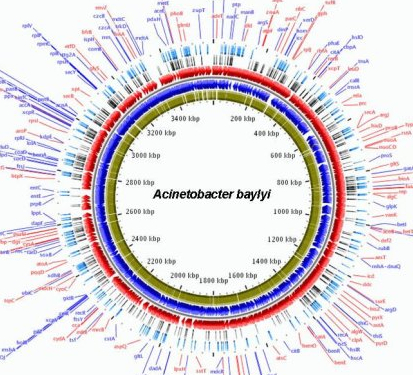
\includegraphics[height=50mm]{acineto}
  \end{center}
  \begin{itemize}[<+-| alert@+>]
    \item Espèce étudiée: \textit{Acinetobacter baylyi}
    \item Taille du génome : $\simeq$ 3 600 000 nucléotides
    \item Lectures longues : Oxford Nanopore (30\% d'erreur) : 89 011, de longueur moyenne $\simeq$ 4 300 nucléotides
  \end{itemize}
\end{frame}
\begin{frame}[fragile]{Résultats : kmersDel et kmersExpand}
  Union des $\textit{k}$-mers + $\textit{k}$-mers à délétion + $\textit{k}$-mers à insertion\medskip\\\pause
  Enormément de $k$-mers inutiles dans les lectures longues (0,23\% à 0,44\% d'utile)\pause
  \begin{itemize}[<+-| alert@+>]
    \item $16$-mers, $freq = 5$, un trou de longueur 1 $\rightarrow 87\%$
    \item $16$-mers, $freq = 5$, un trou de longueur 1 à 2 $\rightarrow 98\%$
  \end{itemize}
  \pause
  Un grand nombre de $\textit{k}$-mers sont trouvés, mais impossible de les filtrer.\medskip\pause\\
  Résultats similaires sur $20$-mers et $11$-mers\medskip\pause\\
  Résultats similaires avec les lectures Pacific Biosciences et Oxford Nanopore.
\end{frame}

\begin{frame}[fragile]{Résultats : Mots Minimaux Absents (MAW)}
  Recherche de Mots Minimaux Absents fréquents :\pause
  \begin{itemize}
    \item Pas concluant, repartition des MAW dans les bons/mauvais $k$-mers trop homogène
  \end{itemize}\pause
  Recherche de Mots Minimaux Absents rares:\pause
  \begin{itemize}
    \item Pas concluant, mêmes résultats que pour les MAW fréquents
  \end{itemize}
\end{frame}

\begin{frame}[fragile]{Résultats : CompaReads\footnote{Nicolas Maillet, Claire Lemaitre, Rayan Chikhi, Dominique Lavenier and Pierre Peterlongo\cite{CompaReads2012}}}
  \textbf{But} : Identifier les lectures longues provenant d'une même région du génome de référence.\medskip\pause\\
  Procédure de test :\pause
  \begin{itemize}[<+-| alert@+>]
    \item Sélection d'une lecture longue
    \item Récupération des lectures longues similaires
    \item Recherche de la lecture longue corrigée correspondante
    \item Vérifier qu'elles s'alignent bien sur la même région du génome
  \end{itemize}\pause
  \textbf{Résultat} : $20$-mers fréquents => 25 lectures longues similaires\medskip\pause\\
  Récupération des lectures longues corrigés correspondantes :\\
  \begin{itemize}
    \item 11 lectures récupérées dont 8 s'alignent sur la même région du génome.
  \end{itemize}\bigskip
\end{frame}

\begin{frame}[fragile]{Résultats : Plus long sous-mot commun (PLSC)}
  Extractions de PLSC entre lectures longues similaires :\pause
  \begin{itemize}[<+-| alert@+>]
    \item Pas d'alignement
    \item 1 lecture brute et son équivalente corrigée $\rightarrow$ mauvais alignement.
    \item 2 lectures corrigées similaires $\rightarrow$ le PLSC s'aligne très bien
  \end{itemize}\pause
  PLSC entre les $k$-mers (32 et 64) des lectures longues similaires :\\
  \begin{itemize}
    \item Pas d'alignement
  \end{itemize}
\end{frame}

\section{Conclusion}
\begin{frame}{Conclusion}
  \begin{itemize}[<+-| alert@+>]
    \item kmersDel et kmersExpand ont obtenus les meilleurs résultats
    \item Marquer les k-mers afin de determiner les zones d'erreurs ou les motifs réguliers
  \end{itemize}
\end{frame}

\begin{frame}[allowframebreaks]{Bibliographie}
  \bibliographystyle{unsrt}
  \bibliography{biblio}
\end{frame}
\end{document}
